\section{Digital-development results and experimental assessment}
\label{sec:results}
\label{sec:deposited_assessment}
\subsection{Two complementary development tasks}
The low-speed case begins with a predefined structure and discovers context-dependent commands. The high-speed case combines structure and dependency discovery. Proprietary structure identifiers, slot assignments and command sequences are withheld. Both pass through coupled fitting, integer-command realization, deployment and deposited-position assessment. A best-found structure is not claimed to be globally optimal.

\subsection{Digital-development coverage and computational evidence}\label{sec:framework_evidence}

The development object is an ordered pair of preceding and current stroke masks, $c=(\vect b^{-},\vect b)$. The required pool $\mathcal C_{\rm req}$ is generated from the declared font, stroke-boundary convention, and baseline cases. For each context, the preceding and current emissions are integrated together, preserving waveform state and particle interactions. Older history is blank and no following stroke is emitted. A rendered message selects the matching ordered context, while the deployed controller selects the corresponding shared lookup address. Local dependency bits specify the control representation; they do not truncate the pair forces in the forward model.

The operating domain is defined before its dependency table. First, specify what must be printed: uppercase A--Z, lowercase a--z, digits 0--9, and the declared punctuation and symbols. Second, enumerate their stroke masks and ordered preceding/current-stroke contexts under the stated boundary convention, adding the isolated and full-stroke baselines. Third, select the dependency labels and bit ordering, project each required context to a controller address, and fit shared commands on that domain. Thus the context pool is derived from the print requirement and history model; the dependency representation is built to serve that pool.

For this declared printable-character set there are 95 glyphs and 224 distinct nonblank font columns. Including the isolated and complete-stroke references gives 235 distinct current-only cases. Introducing the prescribed preceding-stroke contexts yields 644 ordered cases, \emph{including} those 235, rather than adding another 644 to them. The number 644 is specific to this font and finite-history construction, not a universal inkjet constant or the Cartesian product of all binary masks. This is exhaustive coverage of the declared finite operating pool, not of arbitrary text streams, all binary masks, continuous parameter ranges, or all possible structures. The pool determines which shared control entries must be fitted and checked. Unobserved binary lookup addresses remain outside the characterized domain.

For a proposed table, evaluation coverage and acceptance coverage are distinct:
\begin{equation}
 C_{\rm eval}=\frac{|\mathcal C_{\rm evaluated}\cap\mathcal C_{\rm req}|}{|\mathcal C_{\rm req}|},\qquad
 C_{\rm acc}=\frac{|\{c\in\mathcal C_{\rm req}: c\text{ evaluated and accepted}\}|}{|\mathcal C_{\rm req}|}.
\end{equation}
Table~\ref{tab:pool_evidence} reports unchanged deployed integer-command tables evaluated on the full pool at 75 kHz. The declared placement policy is a context vertical RMS no greater than $66.45\um$, a maximum vertical dot error no greater than $132.9\um$, minimum gutter deflection $500\um$, and no missing or merged current targets under the specified event mask. A stricter $10\um$ RMS/$25\um$ maximum diagnostic is also reported. Acceptance depends on this explicit engineering policy and is not a universal print-quality criterion. All errors in this table are computational errors against geometric targets, not errors against measurements.

\begin{table}[htbp]\centering\small\caption{Complete ordered-context pool assessment. Errors are vertical micrometers; Strict uses the tighter diagnostic policy.}\label{tab:pool_evidence}\begin{tabular}{lrrrrr}\toprule Case & Evaluated & Accepted & Strict & Worst RMS & Max. error\\\midrule

Low speed & 644 & 644 & 558 & 14.29 & 22.22 \\

High speed & 644 & 644 & 207 & 55.75 & 122.45 \\

\bottomrule\end{tabular}\end{table}

The complete low- and high-speed assessments took 173.8 and 69.7 seconds, respectively, on an NVIDIA RTX A5000, with compilation reported separately. Both have zero missing or merged current targets. The different structures and native particle-property records make these workload timings, not a controlled causal comparison of structure alone.

\begin{figure}[htbp]\centering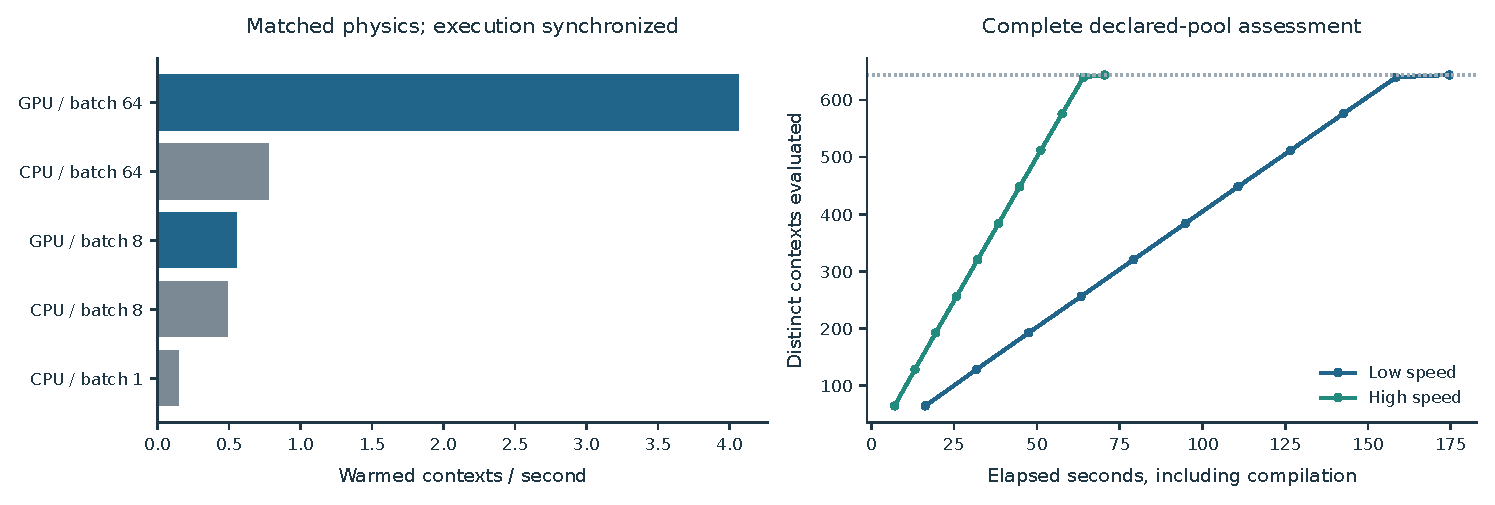
\includegraphics[width=\linewidth]{figures/framework_throughput_coverage.pdf}\caption{Warmed execution throughput and complete-pool evaluation coverage. The acceptance count coincides with the evaluation count for these two tables under the declared policy.}\end{figure}

A current matched batch of 64 low-speed contexts takes 15.66 seconds on the NVIDIA RTX A5000 and 81.45 seconds on the Intel Core i9-14900K CPU, a 5.20-fold warmed execution speedup on this workstation. Compilation/lowering, first execution, warmed execution, transfer and output retention are recorded separately. Particle state is float32 and waveform preparation uses NumPy float64. Two synchronized warm executions are retained; this is a workstation-specific workload result, not a confidence interval or a universal accelerator advantage. The workstation was not reserved exclusively, and background processes and accelerator memory occupancy were not controlled.

\begin{table}[htbp]\centering\small\caption{Consolidated execution evidence. Current rows use the revised executable; archived dense-recording rows retain their original source hash and output contract. Times are seconds.}\label{tab:benchmarks}\begin{tabular}{llrrr}\toprule Workload & Backend & Batch & Compile & Warm median\\\midrule
Industrial endpoints & CPU & 64 & 0.68 & 81.45 \\
Industrial endpoints & GPU & 64 & 1.00 & 15.66 \\
Synthetic endpoints & CPU & 64 & 0.43 & 20.17 \\
Synthetic endpoints & GPU & 64 & 0.68 & 4.38 \\
Archived dense recording & CPU & 1 & 0.60 & 13.59 \\
Archived dense recording & GPU & 1 & 1.00 & 25.37 \\
\bottomrule\end{tabular}\end{table}
The fully specified synthetic benchmark contains 32 spheres of diameter 132 micrometers and density 905 kg/m$^3$, emitted at 75 kHz with initial axial speed 24 m/s. It uses $E_X=-300000$ V/m, independently seeded charge magnitudes uniform on 0.5--1.5 pC (seed 20261111), $h=1$ microsecond and a 4 ms maximum window, with Coulomb and wake/drag terms enabled and coalescence disabled; it contains no industrial font, field or command table. It provides an independently reproducible computational workload, not another physical-validation case. Complete settings, precision, batch shapes, hardware and synchronized timing records are preserved. Application-specific settings are recorded with the reproduction inputs. The archived single-case dense-recording workload returns approximately 1.18 GB and is slower on GPU than CPU, delimiting the acceleration regime. Current matched endpoints and historical dense recording are not compared as identical workloads. The throughput illustration above is retained as the historical reference; the table reports the current rerun.

\paragraph{Effect of development-set coverage.} A controlled coverage-size experiment starts all three fits from the same isolated-flight seed, uses ideal targets and the same bounded update rule and maximum refit passes, and then freezes each table for evaluation on all 644 contexts. The development sets use one glyph, three glyphs, or the complete declared character set. Larger sets cost more; this is not an equal-total-budget optimizer comparison or a new fully converged design campaign. Updates in this intervention are continuous-valued DAC commands; these newly fitted tables have not undergone integer export or printer testing and are separate from the unchanged deployed tables above.

\begin{table}[htbp]\centering\small\caption{Development-set coverage experiment; all frozen tables assessed on the complete pool.}\begin{tabular}{lrrrrr}\toprule Development set & Contexts & Keys (\%) & Accepted & Max. error & Fit (s)\\\midrule

digit 9 & 29 & 14.3 & 563 & 145.2 & 63.7 \\

three glyphs AMO & 53 & 16.7 & 564 & 143.8 & 63.8 \\

all printable ASCII & 644 & 100.0 & 644 & 10.5 & 703.6 \\

\bottomrule\end{tabular}\end{table}

Maximum errors in the intervention table are vertical micrometers. Fit times exclude the common isolated-seed construction and the subsequent frozen full-pool assessment. Unseen entries retain the isolated-row seed rather than receiving a nearest-neighbor or full-font optimized answer. These results characterize this seed and bounded fitting budget; they do not establish a universal relationship between font-set size and final achievable accuracy. Complete-pool fitting and assessment are verification of the intended design domain, not an unseen-context generalization test. The physical assessment instead replays frozen commands without fitting them to the measured coordinates.

\paragraph{Bounded structural exploration.} A separate archived search screened one million surrogate candidates, retained 15,600 unique candidates and selected 512 structures for coupled assessment. The archive contains 3,321 physical-model evaluations, including perturbations and refinements, rather than 3,321 distinct structures. This campaign used a different operating cohort from the two native-75-kHz assessment cases. It demonstrates a staged exploration procedure; it neither exhausts the structural design space nor proves a global optimum. No speedup against an experimental rig or competing search algorithm is inferred from these counts.

\paragraph{Relation to prior optimization studies.} Sato et al.\ report simulation-assisted charging optimization, a five-by-five digit-nine example, printer assessment and a reduction to one seventh of the simulation evaluations used by their MOGA comparator \citep{sato2022}. That reported evaluation-count reduction is not a wall-clock benchmark and is not directly comparable to the CPU/GPU ratio here. Our emphasis is the declared font/history pool, shared controller-table realization and traceable progression from structural screening to complete-pool assessment. We do not infer that their method could not address a larger pool.

\begin{figure}[htbp]\centering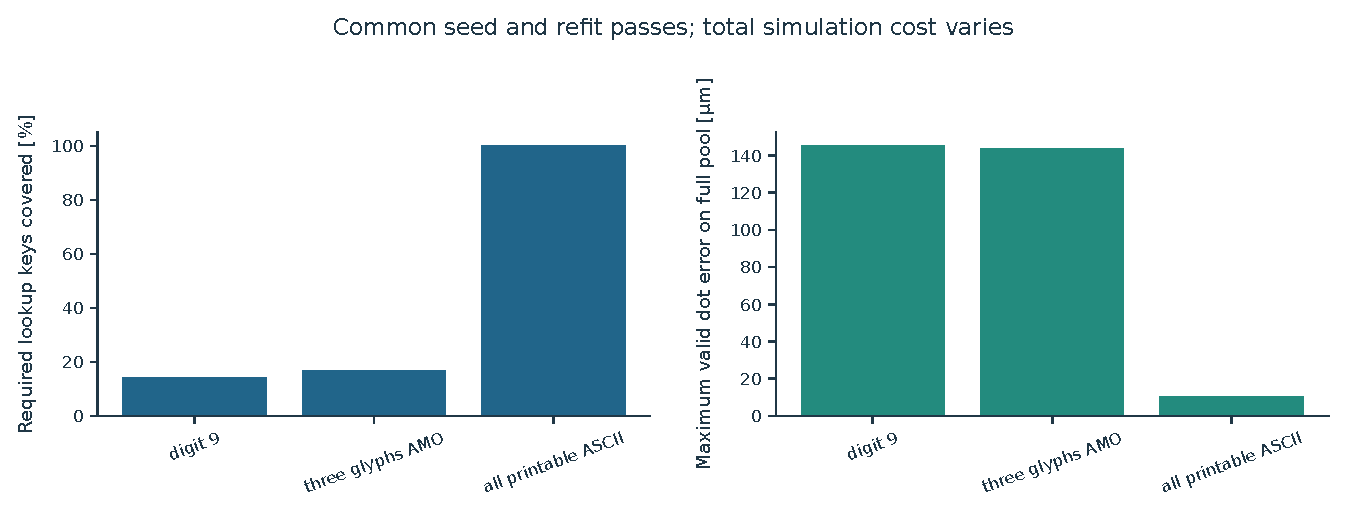
\includegraphics[width=\linewidth]{figures/framework_coverage_intervention.pdf}\caption{Coverage-size intervention from a common isolated-flight seed. All final tables are evaluated on the full pool. Equal refit passes do not imply equal computation time.}\end{figure}

\begin{figure}[htbp]\centering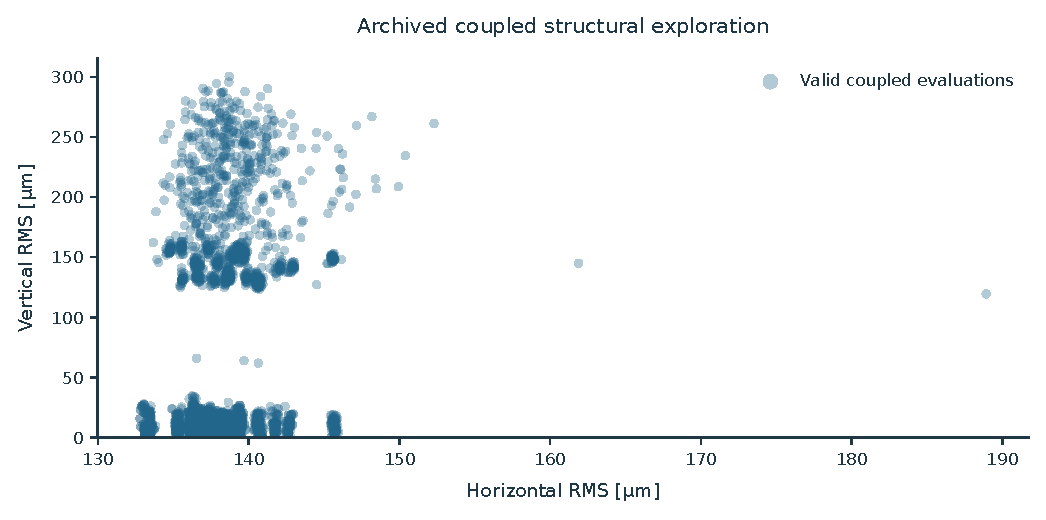
\includegraphics[width=.8\linewidth]{figures/framework_structure_exploration.pdf}\caption{Archived coupled evaluations with valid endpoints, including perturbations and refinements. Endpoint validity alone does not establish all placement and clearance constraints. This separate cohort is not the native-75-kHz experimental assessment.}\end{figure}


\subsection{Operating points and paired measurements}
Computational design was followed by deployment of the resulting DAC table on the printer, physical printing and independent deposited-coordinate extraction. The low-speed case illustrates dependency discovery on a predefined structure. The high-speed case illustrates joint structure and dependency discovery. The main text describes the cases by operating point; the corresponding reproduction inputs are provided with the implementation.

According to the clarified acquisition provenance, ten repeated prints of the same complete uppercase A--Z message were analyzed from images for each raster. Corresponding dot coordinates were averaged across the ten measurements, and the supplied arrays contain these mean positions. There are ten repeated message prints per case; the 26 letters are not treated as independent replicate prints. The collected samples cover uppercase A--Z at 75 kHz and 60 requested horizontal DPI. Substrate speed is 50 m/min for the low-speed case and 100 m/min for the high-speed case. Each supplied coordinate dataset contains 1,725 mean dot positions. Coordinates are in millimeters. A nominal deposited diameter of $528\um$ is used only for footprint visualization; localization error is computed from dot centers.

The low-speed reference is a fresh native-75-kHz physical replay of the unchanged exported integer-DAC table. The high-speed reference uses its native-75-kHz repaired integer-DAC replay. The amplifier and induction sequence are evaluated at that frequency before integrating particle flight. No timing projection substitutes for physical integration, and no commands are refitted to the measured positions. The cached message reconstruction uses previous/current-stroke references with blank older history and no next-stroke emission; it is not an uninterrupted whole-message simulation. The original campaigns also used different native droplet-property records, so this is not a controlled causal comparison of structure alone.

Dot identities are matched by message line, column and logical landing label, rather than nearest-neighbor reassignment. All measured dots are retained. Input hashes, frozen simulation references and derived metrics are preserved in the accompanying repository. The comparison uses a versioned experimental coordinate dataset and fixed simulation predictions; superseded coordinate versions are retained separately and are not pooled as independent acquisitions.

\subsection{Character reconstruction from deposited coordinates}
Figures~\ref{fig:coordinate_low}--\ref{fig:coordinate_high} reconstruct the uppercase glyph samples directly from the paired simulation and measured center coordinates. They are coordinate-based reconstructions, not photographs or newly generated font targets. All 1,725 matched dots per case are retained. Each measured/simulated pair uses identical millimeter scales, bounds and a nominal $528\um$ circular footprint for visual context; actual measured dot diameters are unavailable. The experimental reconstruction depicts mean dot positions across ten prints, rather than any one physical print. Overlay panels show the matched centers at their original relative positions, with no translation, rotation, scale, shear or per-character registration fitted. Letters are displayed in alphabet order; the plotted experimental centers represent the ten-print mean message.

\begin{figure}[p]\centering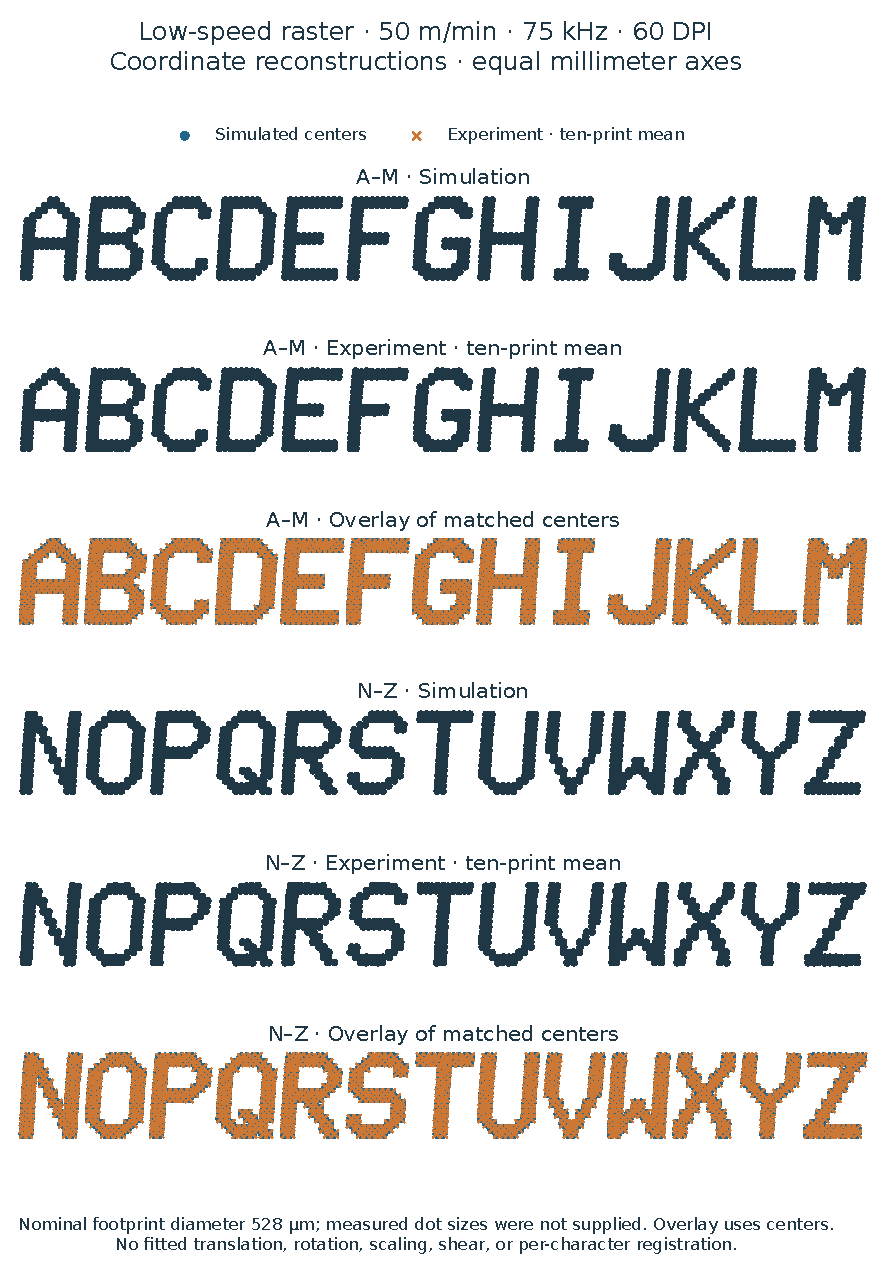
\includegraphics[width=\linewidth,height=0.78\textheight,keepaspectratio]{figures/coordinate_print_low.pdf}\caption{Low-speed case: simulation and measured-print reconstruction from deposited coordinates, followed by matched-center overlays. The same coordinates used for the quantitative errors are shown without an alignment fit. Nominal circle sizes illustrate footprint only.}\label{fig:coordinate_low}\end{figure}
\begin{figure}[p]\centering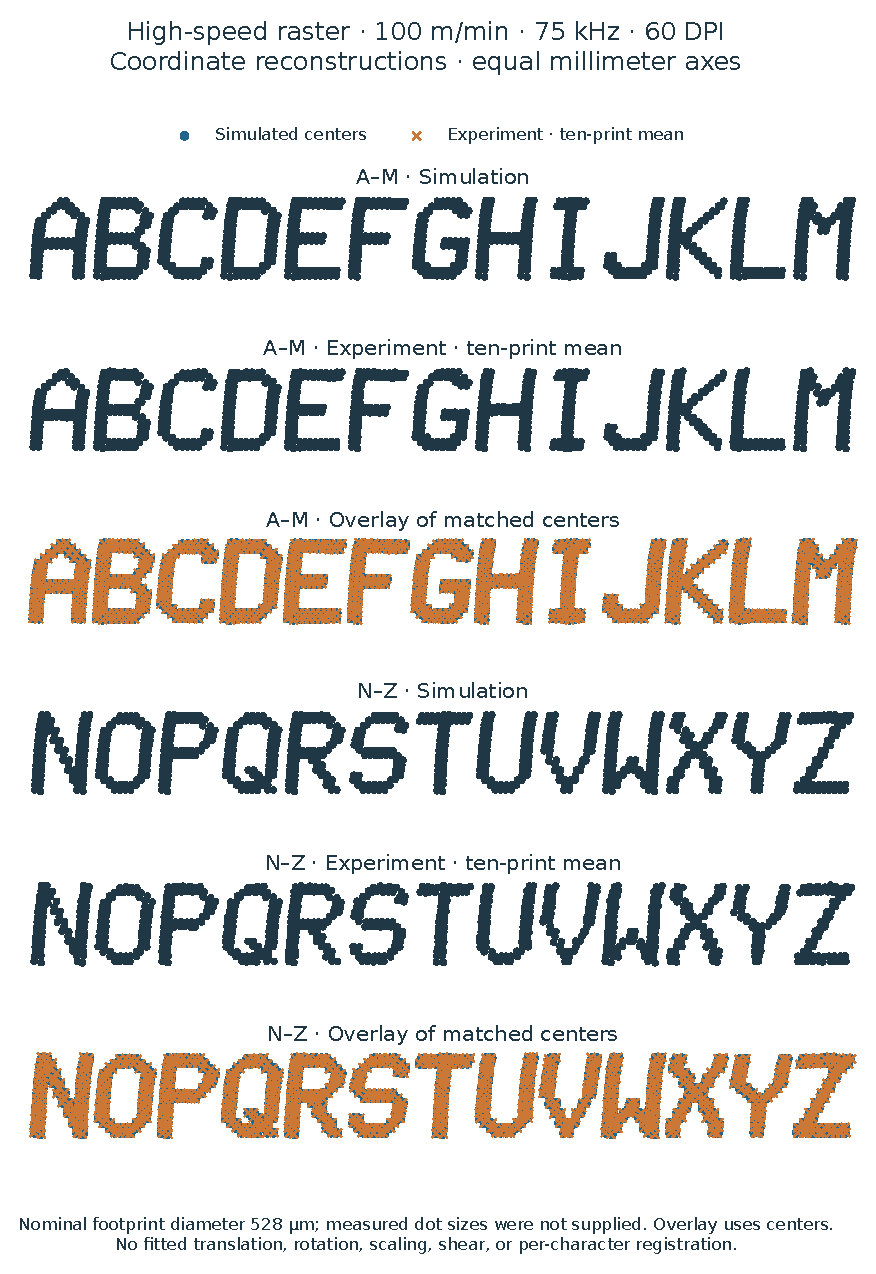
\includegraphics[width=\linewidth,height=0.78\textheight,keepaspectratio]{figures/coordinate_print_high.pdf}\caption{High-speed case: simulation, measured-print reconstruction and matched-center overlays, with equal millimeter axes and all uppercase glyph samples retained.}\label{fig:coordinate_high}\end{figure}
\begin{figure}[htbp]\centering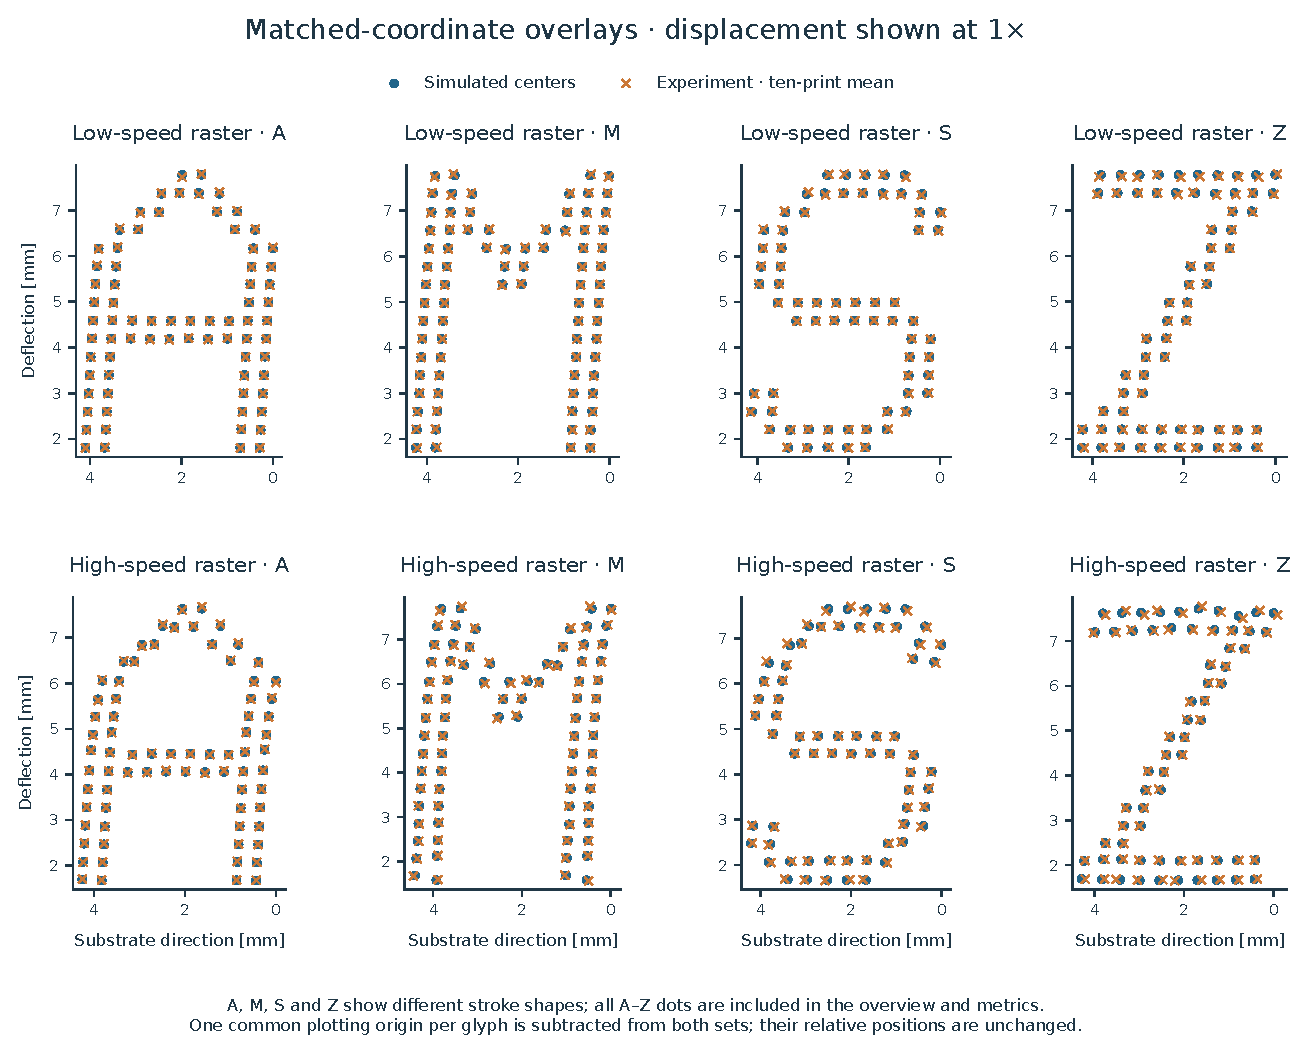
\includegraphics[width=\linewidth]{figures/coordinate_print_closeups.pdf}\caption{Selected character-center overlays at unit displacement scale. Blue dots are simulated centers, orange crosses are measured centers, and gray segments connect matched identities. One identical plotting-origin subtraction is applied to both coordinate sets within each glyph; it does not alter their residuals. These shape examples supplement the complete A--Z views and all-dot metrics.}\label{fig:coordinate_closeups}\end{figure}

\subsection{Prediction accuracy and target quality}
Let $\vect p_i=(y_i,x_i)$ denote the simulated substrate-direction and deflection coordinates, and let $\vect m_i$ denote the corresponding measured position. Prediction residuals and pooled root-mean-square errors are
\begin{equation}
 \vect e_i=\vect m_i-\vect p_i,\quad
 E_a=\sqrt{\frac1n\sum_{i=1}^n e_{i,a}^2},\quad
 E_{2D}=\sqrt{\frac1n\sum_{i=1}^n\lVert\vect e_i\rVert_2^2}.
\end{equation}
These are errors against physical deposited coordinates, distinct from an optimized simulation's residual against an ideal geometric target. A nearly ideal computational print is not itself physical validation.

Table~\ref{tab:deposited_errors} reports raw-coordinate comparisons without fitting translation, rotation, scale, shear, or per-character corrections. The simulator uses one phase defined from its own blank/full-stroke reference, not fitted to measured dots. Whole-file translation and rigid registrations are available separately in the internal sensitivity analysis; those are in-sample nuisance-parameter fits, not additional independent experiments.

\begin{table}[htbp]\centering\small
\caption{Measured-minus-simulated deposited-coordinate errors at the two tested operating points. All errors are in micrometers; P95 refers to radial residual magnitude.}\label{tab:deposited_errors}
\begin{tabular}{lrrrrr}\toprule
Case & Dots & Horizontal RMS & Deflection RMS & 2D RMS & 2D P95\\\midrule
Low speed & 1725 & 20.97 & 16.12 & 26.45 & 50.06 \\
High speed & 1725 & 31.23 & 21.58 & 37.96 & 71.64 \\
\bottomrule\end{tabular}
\end{table}

\begin{figure}[htbp]\centering
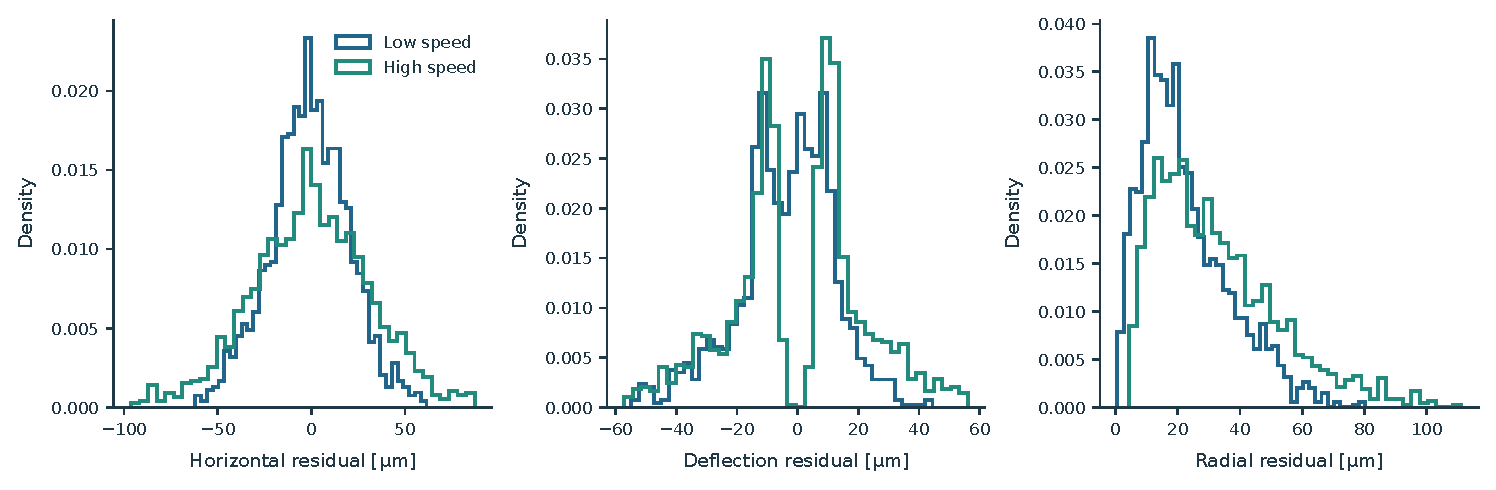
\includegraphics[width=\linewidth]{figures/experimental_residual_distributions.pdf}
\caption{Unregistered residual distributions relative to the experimental mean positions. The cases represent different design tasks and operating points.}
\end{figure}

\begin{figure}[htbp]\centering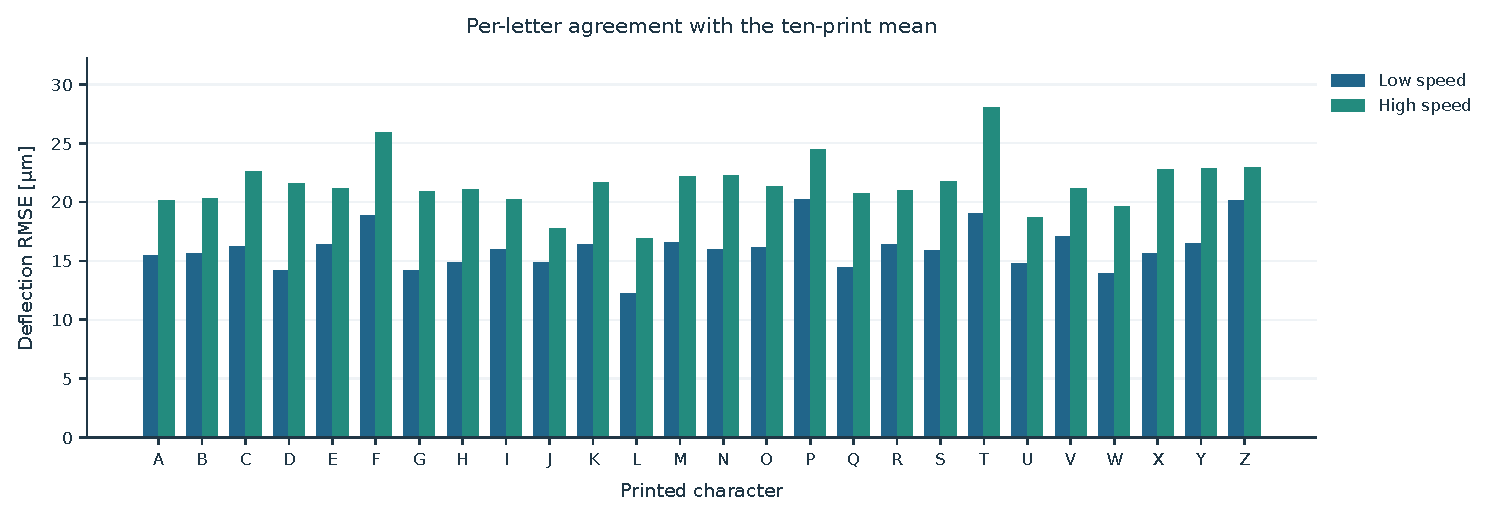
\includegraphics[width=\linewidth]{figures/framework_glyph_assessment.pdf}\caption{Per-character deflection RMSE against the experimental ten-print mean. Commands and coordinate registration are fixed across the assessment.}\label{fig:per_character}\end{figure}

The high-speed case has higher measured-coordinate errors in both directions: 21.58 micrometers RMS in deflection and 31.23 micrometers along substrate motion. Its maximum absolute directional residuals are 57.16 and 96.25 micrometers, respectively. These are prediction discrepancies against the experimental mean positions, separate from the geometric residual minimized during computational design. The commands, field and trajectories were retained for this assessment; no measurement-dependent refit or alignment was applied.

\subsection{Experimental scope and confidentiality}
The released assessment contains 1,725 mean dot positions per raster, obtained from ten repeated A--Z prints at each operating point. Additional laboratory records, including raw images and individual replicate measurements, remain confidential and are outside the public evidence package. The reported RMSE therefore measures disagreement with the released mean coordinates; it does not estimate single-print variability or a repeatability confidence interval.

This assessment tests deposited-position prediction and the computational-to-printer workflow for the two reported configurations. It does not independently identify each force closure or assess intermediate trajectories, contact events or collection margins. Noncoordinate fields retained in the export schema, such as flight time and gutter diagnostics, are simulation metadata rather than additional measured labels. The experimental conclusions are restricted to the released coordinates and operating points.

\subsection{Controlled physics ablation at frozen controller commands}\label{sec:ablation}
The raster commands were developed with the full interacting model. To test whether its in-flight interaction terms matter for those deployed designs, each unchanged integer-command lookup is evaluated with full physics, flight Coulomb forces disabled, wakes disabled, and both disabled. All 644 declared contexts per case are retained. The field, ink properties, charging waveform and induction, guard commands, initial states, event rules, integration step and controller table are identical within each case; no alternative is refitted. In particular, disabling flight Coulomb forces does not disable electrode forces or neighboring-drop charging induction.

The geometric-target assessment and comparison with measured deposited coordinates are distinct. Table~\ref{tab:ablation} reports the full computational pool; Figure~\ref{fig:ablation} compares the A--Z subset with the same measured coordinates and a common simulation-defined phase. Merged targets are not treated as independently localized singleton droplets. Their counts and the number of scoreable measurement pairs are retained, rather than allowing exclusions to improve an ablated model's apparent accuracy.
\begin{table}[htbp]\centering\small
\caption{Fixed-command ablation on 644 contexts per case. RMS is the deflection error of finite requested-target coordinates, including lineage-mapped coordinates; merged targets are separately counted. These are numerical target errors, not measurement RMSE.}\label{tab:ablation}
\begin{tabular}{llrrr}\toprule Case & Physics & Target RMS ($\mu$m) & Accepted contexts & Merged targets\\\midrule
Low & Full & 6.4 & 644 & 0 \\
Low & No flight Coulomb & 51.8 & 484 & 0 \\
Low & No wakes & 103.1 & 69 & 0 \\
Low & Neither & 114.3 & 58 & 0 \\
High & Full & 26.0 & 644 & 0 \\
High & No flight Coulomb & 190.4 & 79 & 524 \\
High & No wakes & 113.2 & 72 & 0 \\
High & Neither & 175.0 & 50 & 0 \\
\bottomrule\end{tabular}\end{table}
\begin{figure}[htbp]\centering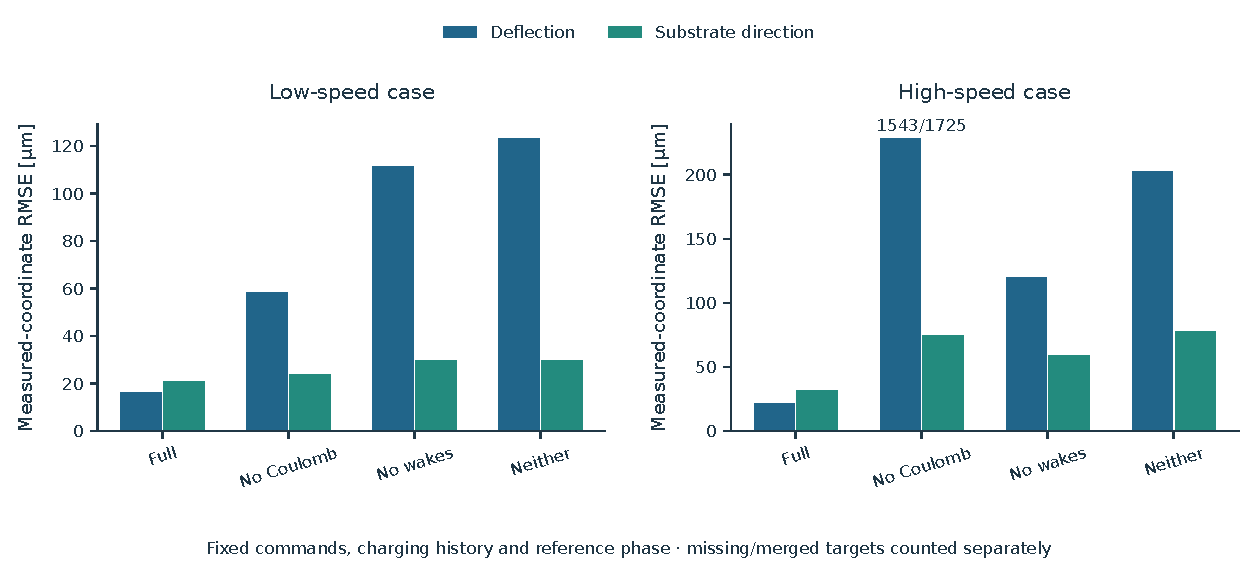
\includegraphics[width=\linewidth]{figures/physics_ablation.pdf}\caption{Coordinate-prediction ablation with unchanged commands and reference phase. Blue and teal bars denote deflection and substrate-direction RMSE. Each case has 1,725 measured target positions; an annotated fraction gives scoreable singletons when merged targets prevent an identity-preserving coordinate comparison.}\label{fig:ablation}\end{figure}
The full model gives the lowest measured deflection RMSE in both cases under this fixed-command test. Its deflection RMSE is 16.1--21.6 micrometers, whereas omitted-term variants span 58.5--228.2 micrometers on their scoreable targets. These results show that the omitted physics matter for the developed command tables. Because those tables were optimized with the full model, this is a conditional deployment/prediction test, not a comparison of independently recalibrated and reoptimized alternatives. It does not uniquely identify each closure or prove that no simplified model could perform adequately after its own development. Coalescence outcomes need not vary monotonically when two coupled terms are removed together.
